\documentclass[fleqn]{article}
\oddsidemargin 0.0in
\textwidth 6.0in
\thispagestyle{empty}
\usepackage{import}
\usepackage{amsmath}
\usepackage{graphicx}
\usepackage{flexisym}
\usepackage{calligra}
\usepackage{amssymb}
\usepackage{bigints} 
\usepackage[english]{babel}
\usepackage[utf8x]{inputenc}
\usepackage{float}
\usepackage[colorinlistoftodos]{todonotes}


\DeclareMathAlphabet{\mathcalligra}{T1}{calligra}{m}{n}
\DeclareFontShape{T1}{calligra}{m}{n}{<->s*[2.2]callig15}{}
\newcommand{\scriptr}{\mathcalligra{r}\,}
\newcommand{\boldscriptr}{\pmb{\mathcalligra{r}}\,}

\definecolor{hwColor}{HTML}{1a0252}

\begin{document}

  \begin{titlepage}

    \newcommand{\HRule}{\rule{\linewidth}{0.5mm}}

    \center

    \begin{center}
      
\includegraphics[height=11cm, width=11cm]{asu.png}
    \end{center}

    \vline

    \textsc{\LARGE Quantum Physics II}\\[1.5cm]

    \HRule \\[0.5cm]
    { \huge \bfseries Problem Set Five}\\[0.4cm] 
    \HRule \\[1.0cm]

    \textbf{Behnam Amiri}

    \bigbreak

    \textbf{Prof: Onur Erten}

    \bigbreak

    \textbf{{\large \today}\\[2cm]}

    \vfill

  \end{titlepage}

  \textbf{Background Information}
  \\
  \\
  \textcolor{hwColor}{
    Suppose that $S$ is a bounded region in $\mathbb{R}^3$, which has volume $V>0$, and that $f(x, y, z)$ 
    is a real-valued function, which is Riemann integrable on $S$, then the average value of $f$ on $S$ is
    $$
      \dfrac{1}{V} \bigintsss \bigintsss\limits_{S} \bigintsss f(x, y, z) ~ dV
    $$
    In Quantum mechanical calculation the expectation value is defined as
    $$
      \langle x \rangle=\bigintsss\limits_{-\infty}^{+\infty} x \psi(x, t) \psi^*(x, t) dx
    $$
    This integral can be interpreted as the average value of x that we would expect to obtain from a large number 
    of measurements. Alternatively it could be viewed as the average value of position for a large number of particles 
    which are described by the same wavefunction. For example, the expectation value of the radius of the 
    electron in the ground state of the hydrogen atom is the average value you expect to obtain from making 
    the measurement for a large number of hydrogen atoms.
    \\
    For the Hydrogen atom, we have an electron which is loacted at some distance $r$ from the origin. 
    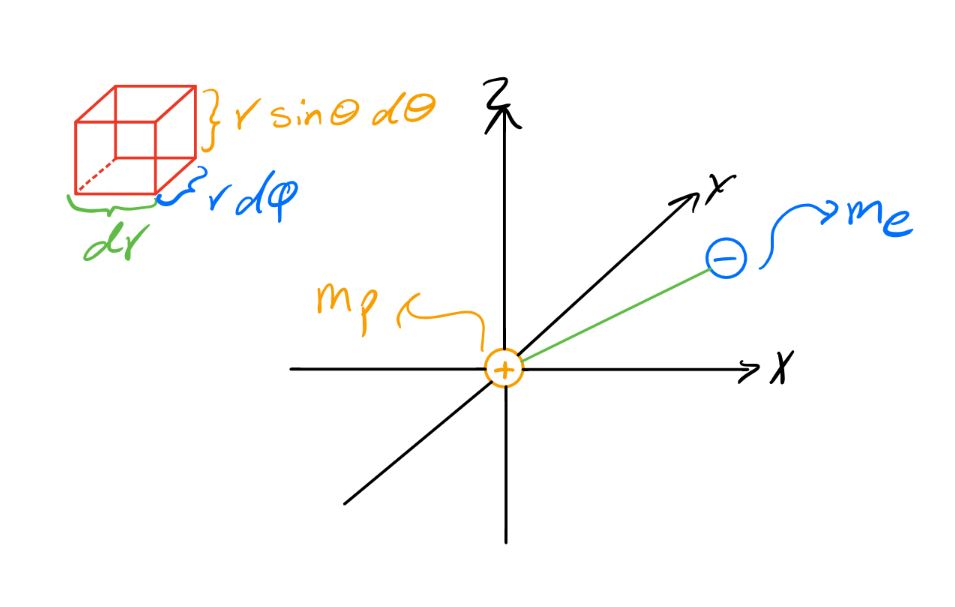
\includegraphics[height=3cm, width=5cm]{One.JPG}
    \\
    Our goal is calculating the average radius that the electron moves around. The following equation does the job for us.
    $$
      \langle W \rangle=\bigintsss\limits_{0}^{2\pi} d\phi 
      ~ \bigintsss\limits_{0}^{\pi} sin(\theta) d\theta 
      ~ \bigintsss\limits_{0}^{\infty} W dr ~ r^2 \psi^*(r, \theta, \phi) \psi(r, \theta, \phi) 
    $$
    Given that the hydrogen atom contains a nucleus and an electron, quantum mechanics allows one to predict the probability of finding the electron at 
    any given radial distance $r$. It is given by the square of a mathematical function known as the \emph{wavefunction} which is a 
    solution of the Schr$\ddot{o}$dinger equation. The lowest energy equilibrium state of the hydrogen atom is known as the ground state.
    \\
    Page 148 of the textbook states the ground state of hydrogen as $\psi_{1, 0, 0}(r, \theta, \phi)=\dfrac{1}{\sqrt{\pi a^3}} e^{-r/a}$
    where $a=\dfrac{4 \pi \epsilon_0 \hbar^2}{m_e e^2}$ is the Bohr radius.
    \\
  } 

  \begin{enumerate}
    \item \textbf{4-15}
    \begin{enumerate}
      \item Find $\langle r \rangle$ and $\langle r^2 \rangle$ for an electron in the ground state of hydrogen. Express your
      answers in terms of the Bohr radius. 

        \textcolor{hwColor}{
          \\
          $
            \langle r \rangle=\bigints\limits_{0}^{2\pi} 
            ~ \bigints\limits_{0}^{\pi} 
            ~ \bigints\limits_{0}^{\infty} ~ r ~ \psi^*_{100} \psi_{100} ~ r^2 sin(\theta) dr ~ d\theta ~ d\phi
            \\
            \\
            \\
            =\bigints\limits_{0}^{2\pi} d\phi
            ~ \bigints\limits_{0}^{\pi} sin(\theta) d\theta 
            ~ \bigints\limits_{0}^{\infty} r^3 ~ \dfrac{1}{\sqrt{\pi a^3}} e^{-r/a} ~ \dfrac{1}{\sqrt{\pi a^3}} e^{-r/a} dr
            \\
            \\
            \\
            =\left(2 \pi\right).\left(2\right).\dfrac{1}{\pi a^3} \bigints\limits_{0}^{\infty} r^3 e^{-2r/a} ~ dr
            \\
            \\
            \\
            =\left(2 \pi\right).\left(2\right).\left(\dfrac{1}{\pi a^3} \dfrac{3!}{(2/a)^{3+1}}\right)
            \\
            \\
            \\
            \therefore ~~~ \langle r \rangle=\dfrac{3}{2}a ~~~~~ \checkmark
            \\
            \\
            \\
            \\
            \\
            \langle r^2 \rangle=\bigints\limits_{0}^{2\pi} 
            ~ \bigints\limits_{0}^{\pi} 
            ~ \bigints\limits_{0}^{\infty} ~ r^2 ~ \psi^*_{100} \psi_{100} ~ r^2 sin(\theta) dr ~ d\theta ~ d\phi
            \\
            \\
            \\
            =\bigints\limits_{0}^{2\pi} d\phi
            ~ \bigints\limits_{0}^{\pi} sin(\theta) d\theta 
            ~ \bigints\limits_{0}^{\infty} r^4 ~ \dfrac{1}{\sqrt{\pi a^3}} e^{-r/a} ~ \dfrac{1}{\sqrt{\pi a^3}} e^{-r/a} dr
            \\
            \\
            \\
            =\left(2 \pi\right).\left(2\right).\dfrac{1}{\pi a^3} \bigints\limits_{0}^{\infty} r^4 e^{-2r/a} ~ dr
            \\
            \\
            \\
            =\left(2 \pi\right).\left(2\right).\left(\dfrac{1}{\pi a^3} \dfrac{4!}{(2/a)^{4+1}}\right)
            \\
            \\
            \\
            \therefore ~~~ \langle r^2 \rangle=3a^2 ~~~~~ \checkmark
          $
        }

      \pagebreak

      \item Find $\langle x \rangle$ and $\langle x^2 \rangle$ for an electron in the ground state of hydrogen. 
      \emph{Hint: This requires no new integration-note that $r^2=x^2+y^2+z^2$, and exploit the symmetry of the ground state}

        \textcolor{hwColor}{
          \\
          We know that in the Spherical coordinate system we have
          $$
            \begin{cases}
              x=r sin(\theta) cos(\phi)
              \\
              y=r sin(\theta) sin(\phi)
              \\
              z=r cos(\theta)
            \end{cases}
          $$
          Therefore,
          \\
          \\
          $
            \langle x \rangle=\bigints\limits_{0}^{2\pi} 
            ~ \bigints\limits_{0}^{\pi} 
            ~ \bigints\limits_{0}^{\infty} ~ x ~ \psi^*_{100} \psi_{100} ~ r^2 sin(\theta) dr ~ d\theta ~ d\phi
            \\
            \\
            \\
            =\bigints\limits_{0}^{2\pi} 
            ~ \bigints\limits_{0}^{\pi} 
            ~ \bigints\limits_{0}^{\infty} 
            ~ \left(r sin(\theta) cos(\phi)\right) 
            ~ \left(\dfrac{1}{\sqrt{\pi a^3}} e^{-r/a} . \dfrac{1}{\sqrt{\pi a^3}} e^{-r/a}\right) 
            ~ r^2 sin(\theta) dr ~ d\theta ~ d\phi
            \\
            \\
            \\
            =\dfrac{1}{\pi a^3} \bigints\limits_{0}^{2\pi} cos(\phi) d\phi 
            ~ \bigints\limits_{0}^{\pi} sin^2(\theta) d\theta
            ~ \bigints\limits_{0}^{\infty} r^3 e^{-2r/a} dr
            \\
            \\
            \\
            \\
            \\
            \bigints\limits_{0}^{2 \pi} cos(\phi) d\phi=sin(\theta) \Big|_{0}^{2 \pi}=sin(2 \pi)-sin(0)=0 ~~~~ \checkmark
            \\
            \\
            \\
            \\
            \\
            \langle x \rangle=0 
            ~ \bigints\limits_{0}^{\pi} sin^2(\theta) d\theta
            ~ \bigints\limits_{0}^{\infty} r^3 e^{-2r/a} dr
            \\
            \\
            \\
            \therefore ~~~ \langle x \rangle=0 ~~~~ \checkmark
          $
          \\
          \\
          This integral is zero because we are integrating an odd function over a symmetric region. $\langle x \rangle$ is the 
          average position of an electron on the x-axis, because $x=r sin(\theta) cos(\phi)$ is the conversion from Spherical to 
          Cartesian coordinates. This result tells us that the average position is $0$.
          \\
          \\
          \\
          $
            \langle x^2 \rangle=\bigints\limits_{0}^{2\pi} 
            ~ \bigints\limits_{0}^{\pi} 
            ~ \bigints\limits_{0}^{\infty} ~ x^2 ~ \psi^*_{100} \psi_{100} ~ r^2 sin(\theta) dr ~ d\theta ~ d\phi
            \\
            \\
            \\
            =\bigints\limits_{0}^{2\pi} 
            ~ \bigints\limits_{0}^{\pi} 
            ~ \bigints\limits_{0}^{\infty} 
            ~ \left(r sin(\theta) cos(\phi)\right)^2 
            ~ \left(\dfrac{1}{\sqrt{\pi a^3}} e^{-r/a} . \dfrac{1}{\sqrt{\pi a^3}} e^{-r/a}\right) 
            ~ r^2 sin(\theta) dr ~ d\theta ~ d\phi
            \\
            \\
            \\
            =\dfrac{1}{\pi a^3} \bigints\limits_{0}^{2\pi} cos^2(\phi) d\phi
            ~ \bigints\limits_{0}^{\pi} sin^3(\theta) d\theta
            ~ \bigints\limits_{0}^{\infty} r^4 e^{-2r/a} dr
            \\
            \\ 
            \\
            =\dfrac{1}{\pi a^3} \left[
              \left(\dfrac{\phi}{2}+\dfrac{sin(2\phi)}{4}\right) \Big|_{0}^{2 \pi}
              \left(-cos(\theta)+\dfrac{cos^3(\theta)}{3}\right) \Big|_{0}^{\pi}
              \left(\dfrac{4!}{(2/a)^{4+1}}\right)
            \right]
            \\
            \\
            \\
            =\dfrac{1}{\pi a^3} \left[
              (\pi).
              (\dfrac{4}{3}).
              (\dfrac{24 a^5}{32})
            \right]
            \\
            \\
            \\
            \therefore ~~~ \langle x^2 \rangle=a^2 ~~~~ \checkmark
          $
          \\
          \\
          For $x^2$ we see that $x$ is an arbitrary direction meaning $x, y$ and $z$ have equal weights. Therefore, we can say that 
          the expectation value of $x^2$ is one third of the expectation value of $r^2$. We also see that the expectation value of 
          $x^2$ does not produce an odd function hence it will not be zero.
          \\
        }


      \item Find $\langle x^2 \rangle$ in the state $n=2$, $\ell=1$, $m=1$. \emph{Hint: this state is not symmetrical in 
      $x, y,z.$ Use $x=r sin(\theta) cos(\phi)$.}

        \textcolor{hwColor}{
          \\
          By consulting the textbook we know that $\psi_{2, 1, 1}(r, \theta, \phi)=\dfrac{1}{8\sqrt{\pi a^3}} \dfrac{r}{a} e^{-r/2a} sin(\theta) e^{i \theta}$. Therefore,
          \\
          $
            \langle x^2 \rangle=\bigints\limits_{0}^{2\pi} 
            ~ \bigints\limits_{0}^{\pi} 
            ~ \bigints\limits_{0}^{\infty} ~ x^2 ~ \psi^*_{211} \psi_{211} ~ r^2 sin(\theta) dr ~ d\theta ~ d\phi
            \\
            \\
            \\
            =\bigints\limits_{0}^{2\pi} 
            ~ \bigints\limits_{0}^{\pi} 
            ~ \bigints\limits_{0}^{\infty} ~ \left(r sin(\theta) cos(\phi)\right)^2 
            ~ \left[
              \dfrac{1}{8\sqrt{\pi a^3}} \dfrac{r}{a} e^{-r/2a} sin(\theta) e^{-i \theta} \psi_{211} 
              ~ \dfrac{1}{8\sqrt{\pi a^3}} \dfrac{r}{a} e^{-r/2a} sin(\theta) e^{i \theta}
            \right]
            ~ r^2 sin(\theta) dr ~ d\theta ~ d\phi
            \\
            \\
            \\
            =\dfrac{1}{64 \pi a^5}
            \bigints\limits_{0}^{2\pi} cos^2(\phi) e^{i \phi} e^{-i \phi} d\phi
            ~ \bigints\limits_{0}^{\pi} sin^5(\theta) d\theta
            ~ \bigints\limits_{0}^{\infty} r^6 e^{-r/a} dr
            \\
            \\
            \\
            =\dfrac{1}{64 \pi a^5}
            \left[
              \left(\dfrac{\phi}{2}+\dfrac{sin(2\phi)}{4}\right) \Big|_{0}^{2 \pi}
              .\left(-cos(\theta)+\dfrac{2 cos^3(\theta)}{3}-\dfrac{cos^5(\theta)}{5}\right) \Big|_{0}^{\pi}
              .\left(\dfrac{6!}{(1/a)^{6+1}}\right)
            \right]
            \\
            \\
            \\
            =\dfrac{1}{64 \pi a^5}  \left[
              \pi
              .\dfrac{16}{15}
              .720 a^7
            \right]
            \\
            \\
            \\
            \therefore ~~~ \langle x^2 \rangle=12a^2 ~~~~ \checkmark
            \\
          $
        }


    \end{enumerate}

    \item \textbf{4-15} What is the \emph{most probable} value of $r$, in the ground state of hydrogen? 
    (The answer is \emph{not zero!}) \emph{Hint:} First you must figure out the probablity that the electron would be found between
    $r$ and $r+dr$.

      \textcolor{hwColor}{
        \\
        Recall that the state of a quantum object is completely specified by a wavefunction denoted as $\psi(x)$. The probability 
        density (or probably distribution) is given by taking the square of the absolute value of the wave function. It gives us 
        the likelihood of finding an electron (or some other system) at some given point in space. The question is why do we need 
        to take the square of the absolute value of the wave function? Shouldn't the wave function itself be able to tell us 
        the probability? Although the wave function itself does indeed tell us the probability amplitude of the wave produced, 
        it usually is given by some complex value with imaginary numbers and therefore does not hold any true physically measurable 
        meaning. To rid the wave function of its imaginary numbers, we need to take the square of the absolute value which does 
        in fact produce a measurable and meaningful number. 
        \\
        By starting off with the wavefunction of the ground state which is $\psi_{100}=\dfrac{1}{\sqrt{\pi a^3}} e^{-r/a}$, we have:
        \\
        \\
        For a sphere we have:
        \\
        \\
        $
          V=\dfrac{4}{3} \pi r^3 \Longrightarrow \dfrac{dV}{dr}=\dfrac{4}{3} \pi \dfrac{d}{dr}(r^3)
          \\
          \\
          \\
          \therefore ~~~ dV=4 \pi r^2 dr ~~~~ \checkmark ~~~~ \text{The spherical volume element between $r$ and $r+dr$}
        $
        \\
        \\
        \\
        $
          |\psi_{100}|^2=\left(\dfrac{1}{\sqrt{\pi a^3}} e^{-r/a}\right)^2=\dfrac{1}{\pi a^3} e^{-2r/a}
          \\
          \\
          \\
          P(r) dr=|\psi_{100}|^2 dV=|\psi_{100}|^2 4 \pi r^2 dr
          \\
          \\
          \\
          \therefore ~~~ P(r)=4 \pi r^2 |\psi_{100}|^2=4 \pi r^2 ~ \dfrac{1}{\pi a^3} e^{-2r/a}
        $
        \\
        \\
        \\
        \\
        \\
        We can use calculus to find the value of $r$ such that $P(r)$ is at its max. By equating the derivative 
        of $P(r)$ with respect to $r$ to zero, we can find the maximum probable value. (The maxima)
        \\
        \\
        \\
        $
          \dfrac{dP(r)}{dr}=\dfrac{d}{dr} \left(4 \pi r^2 ~ \dfrac{1}{\pi a^3} e^{-2r/a}\right)
          =\dfrac{4}{a^3} \dfrac{d}{dr} \left(r^2 e^{-2r/a}\right)
          \\
          \\
          \\
          =\dfrac{4}{a^3} \left[
            2r e^{-2r/a}-\left(\dfrac{2}{a}\right) e^{-2r/a} r^2
          \right]
          \\
          \\
          \\
          \dfrac{dP(r)}{dr}=0 \Longrightarrow \dfrac{4}{a^3} \left[
            2r e^{-2r/a}-\left(\dfrac{2}{a}\right) e^{-2r/a} r^2
          \right]=0
          \\
          \\
          \\ 
          r e^{-2r/a}-\dfrac{r^2}{a} e^{-2r/a}=0
          \\
          \\
          \\
          1=\dfrac{r^2}{a} 
          \\
          \\
          \\
          \therefore ~~~ r=a ~~~~ \checkmark
        $
      }


  \end{enumerate}

\end{document}




% dV=4πr2dr can be thought of as the spherical volume element between r and r+dr.